\subsection{Gantt Chart} \label{subsec:gantt}
A Gantt chart is generated based on the UPPAAL \gls{cora} schedule, an example of this can be seen in \cref{fig:gantt}. From the Gantt chart the user will be able to see when the individual payloads will be executed, additionally the insolation periods, and windows that specifies when some payloads are allowed to be executed, in is shown in the chart to help the user get a better understanding of the schedule and how the payloads are executed accordingly to their respective windows. On the right side of the chart, information about the different coloured bars, are shown, they represent the payloads, insolation periods, and windows. 

We have decided to not represent the SoC on the chart, since the UPPAAL \gls{cora} model uses the linear battery model. We believe it may be miss leading as the battery model is imprecise.
%Likewise the UPPAAL \gls{smc} model is not a one-to-one representation of the UPPAAL \gls{cora} schedule due to its potential difference in execution lengths it will also not be a good representation of the battery levels during the schedule if their are compared to the UPPAAL \gls{cora} schedule.

\begin{figure}[!h]
	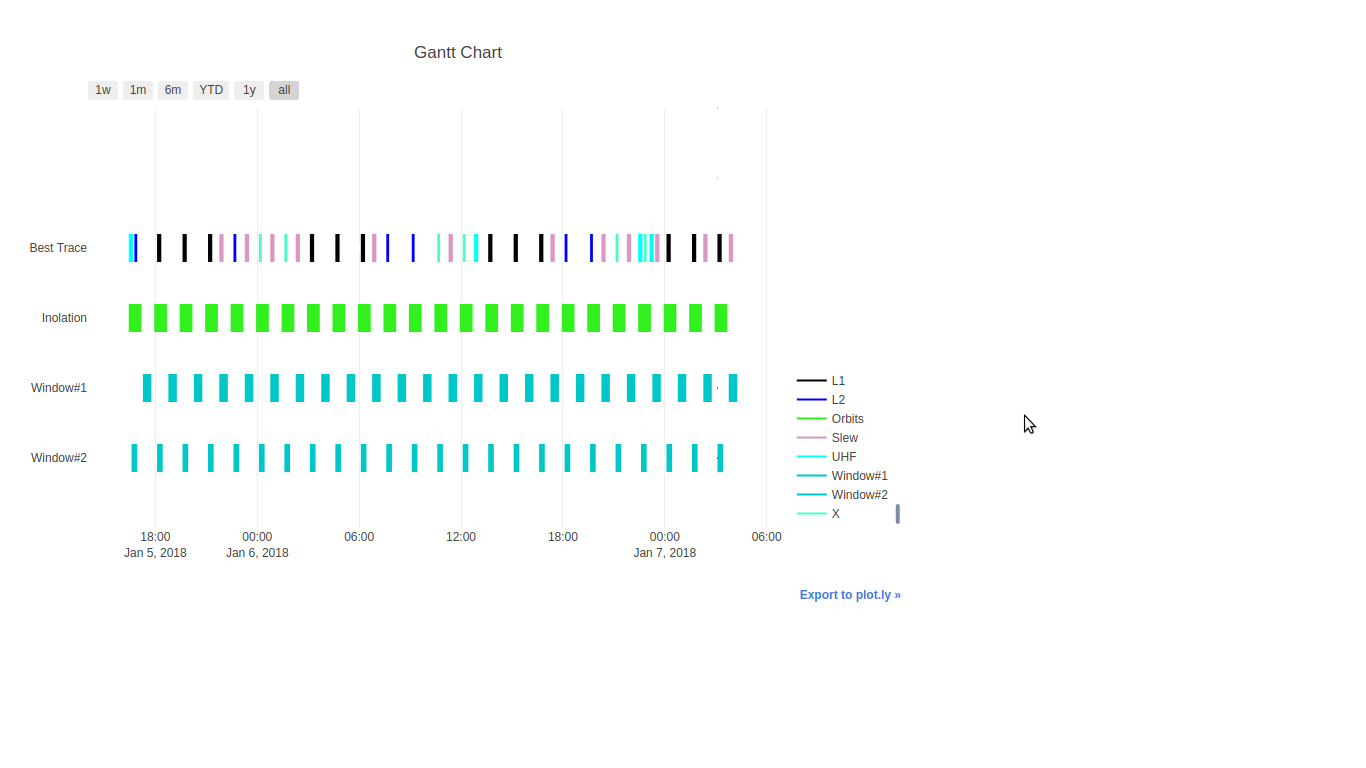
\includegraphics[width=\textwidth]{graphics/gantt.png}
	\caption{A graphical representation of the \gls{cora} schedule}
	\label{fig:gantt}
\end{figure}
The chart will be produced even if the robustness verification fails to accept the schedule. The user will therefore have acces to all of the charts throughout the iteration. By doing so, the user may analyse the charts to better figure out if the want to accept the schedules or if they want to adjust some of the payloads or parameters themselves.
